\documentclass{article}
\usepackage[utf8]{inputenc}
\usepackage[usenames,dvipsnames,pdftex]{xcolor}
\usepackage{fullpage}
\usepackage[upright]{fourier}
\usepackage{tkz-graph}
\usetikzlibrary{arrows}
\begin{document}
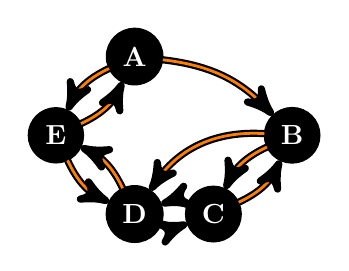
\begin{tikzpicture}[>=stealth']
    \tikzset{node distance = 3cm}
    \tikzstyle{VertexStyle}=[shape        = circle,
                             fill         = black,
                             minimum size = 20pt,
                             text         = white,
                             draw]
    \tikzstyle{TempStyle}=[double           = orange,
                           double distance  = 1pt]
    \Vertex[L= {\textbf{E}}]{E}
    \NOEA[L  = {\textbf{A}}](E){A}
    \SOEA[L  = {\textbf{D}}](E){D}
    \EA[L    = {\textbf{C}}](D){C}
    \NOEA[L  = {\textbf{B}}](C){B}
    \tikzstyle{EdgeStyle}=[TempStyle,
                           ->,
                           bend right      = 20]
    \Edges(A,E,D,C,B)
    \tikzstyle{EdgeStyle}=[TempStyle,
                           ->,
                           bend right      = 30]
    \Edges(B,D)
    \tikzstyle{EdgeStyle}=[TempStyle,
                           <-,
                           bend right      = 20]
    \Edges(B,A) 
    \tikzstyle{EdgeStyle}=[TempStyle,
                           <-,
                           bend left       = 20]
    \Edges(A,E,D,C,B)
\end{tikzpicture}
\end{document}
% Author : Alain Matthes
% Encoding : UTF8
% Engine : PDFLaTeX
